\documentclass{article}
\usepackage{fullpage}
\usepackage{times}
\usepackage{graphicx}
\usepackage{colortbl}
\usepackage{tabto}
\usepackage[table]{xcolor}
\usepackage{subcaption}
\usepackage[font=footnotesize,labelfont=bf]{caption}

\usepackage[bookmarks,
  bookmarksopen = true,
  bookmarksnumbered = true,
  breaklinks = true,
  colorlinks = true,
  linkcolor = black,
  urlcolor  = black,
  citecolor = black,
  anchorcolor = green,
  hyperindex = true,
  hyperfigures
]{hyperref}

\begin{document}


\begin{figure}[t]
  \centering
  
\includegraphics[width=0.4\textwidth]{images/logo.png}
\end{figure}

\title{Machine Learning project on Titanic}

%Insert your name and ID inside the brackets
\author{Davide Ligari 518592}
\date{\today}


\maketitle

\clearpage
\setcounter{page}{1}


%Figures and tables must be cited in the text and explained in detail. Do not forget to add a caption to each figure/table/
\tableofcontents
\clearpage
\section{Introduction}
The sinking of the Titanic remains one of the most notorious maritime disasters in history.
The tragic incident occurred on April 15, 1912, when the supposedly "unsinkable" RMS Titanic collided with an iceberg on its first voyage.
Despite the efforts of the crew, there were not enough lifeboats to accommodate all 2224 passengers and crew members, resulting in the deaths of 1502 people.
While luck played a role in determining who survived the disaster, certain groups of people were more likely to make it out alive than others.
Further investigation reveals that not all passengers had an equal chance of survival, and factors such as age, gender, social class,
and proximity to lifeboats played a significant role in determining one's fate.
The data of some passengers have been collected and are used in this project to check whether the passengers had the same probability to survive or not.

\subsection{Train and test datasets}
The information pertaining to 887 passengers has been gathered and subsequently split into two distinct sets: a training set and a test set.
The test set consists of 177 cases, the training one comprises 710 samples.
The train set is bigger than the test one because it is used in the training phase, and the accuracy of the model is highly related to its size.
On the contrary, the test set is used only to evaluate the quality of the model.
All datasets are available in two distinct text files, which contain the following information about the passengers:

\begin{enumerate}
  \item The ticket class (1st, 2nd or 3rd)
  \item Sex (0 → male, 1 → female)
  \item Age in years
  \item Number of siblings and spouses aboard
  \item Number of parents and children aboard
  \item The passenger fare.
  \item Whether the passenger survived (1) or not (0)
\end{enumerate}

\noindent
Below an example of how the data are organized into the files:
\bgroup
\rowcolors{2}{green!8}{green!18}

\begin{table}[h]
  \center
  \begin{tabular}{ccccccc}
    Class & Sex & Age & N siblings & N parents & Fare    & Survived \\
    \hline
    1     & 1   & 19  & 0          & 0         & 30      & 1        \\
    3     & 0   & 61  & 0          & 0         & 6.2375  & 0        \\
    3     & 0   & 35  & 0          & 0         & 7.05    & 0        \\
    3     & 0   & 45  & 0          & 0         & 6.975   & 0        \\
    3     & 0   & 9   & 4          & 2         & 31.3875 & 0        \\
    3     & 1   & 21  & 2          & 2         & 34.375  & 0        \\
    1     & 0   & 27  & 0          & 2         & 211.5   & 0        \\
    1     & 1   & 35  & 1          & 0         & 83.475  & 1        \\
    1     & 1   & 18  & 2          & 2         & 262.375 & 1        \\
    3     & 0   & 20  & 0          & 0         & 7.8958  & 0        \\
    2     & 0   & 25  & 0          & 0         & 13      & 0        \\
    3     & 1   & 22  & 0          & 0         & 7.775   & 1        \\
    1     & 0   & 37  & 0          & 1         & 29.7    & 0        \\
    3     & 0   & 20  & 8          & 2         & 69.55   & 0        \\
    3     & 0   & 33  & 1          & 1         & 20.525  & 0        \\
  \end{tabular}
  \label{table:titainc_passengers}
  \caption{Example of the information collected about the passengers}
\end{table}
\egroup
\clearpage
\subsection{Logistic regression}
Logistic regression is a well-known classification method.
In this project it is used to predict whether a new passenger survived or not.
So, it calculates the probability of surviving of new passenger and
if it is higher than 0.5 the passenger survived (model returns 1),
otherwise, he died (model returns 0).
The probability is calculated through the sigmoid function:


\begin{equation}\label{Sigmoid}
  \hat{p_i}= \frac{1}{1+e^{-z_i}}
\end{equation}

\noindent
Where z is the logit :

\begin{equation}\label{logit}
  z_i = \omega x_i + b
\end{equation}
\noindent
The optimal values of $ \omega$ and b are the ones that minimize the average of the negative loglikelihood :

\begin{equation}\label{nloglikelihood}
  min \frac{1}{m}\sum_{i=0}^{n-1} -y_i\log{\hat{p_i}}-(1-y_i)\log{(1-\hat{p_i})}\end{equation}


\noindent
Since the loglikelihood is not linear in $ \omega$ and b, it cannot be minimized analytically,
but it is necessary to apply an iterative method, like gradient descent.
This algorithm, at each iteration, calculates the parameters
(formulae \ref*{paramsOmega} , \ref*{paramsB}) and after a certain number of steps it found the weights that minimize the crossentropy.





\begin{equation}\label{paramsOmega}
  \omega^{i+1}= w^i -\eta(\frac{1}{m}X^T(\hat{P}-Y))
\end{equation}

\begin{equation}\label{paramsB}
  b^{i+1}= b^i -\frac{\eta}{m}\sum_{i=0}^{m-1}(\hat{p_i}-y_i)
\end{equation}

\clearpage

\section{Train a model}
\subsection{Which is a good value for the learning rate?}
Since there is not a defined procedure to calculate the best value of the learning rate,
the model has been trained with different values (from $10^{-5}$ to 1) and it is selected
the value that maximizes the accuracy or minimizes the loss function with the lowest number of iterations.
As shown in the figure \ref*{fig:three_images}, the optimal learning rate is 0.001



\begin{figure}[h]
  \centering
  \begin{subfigure}{0.3\linewidth}
    \centering
    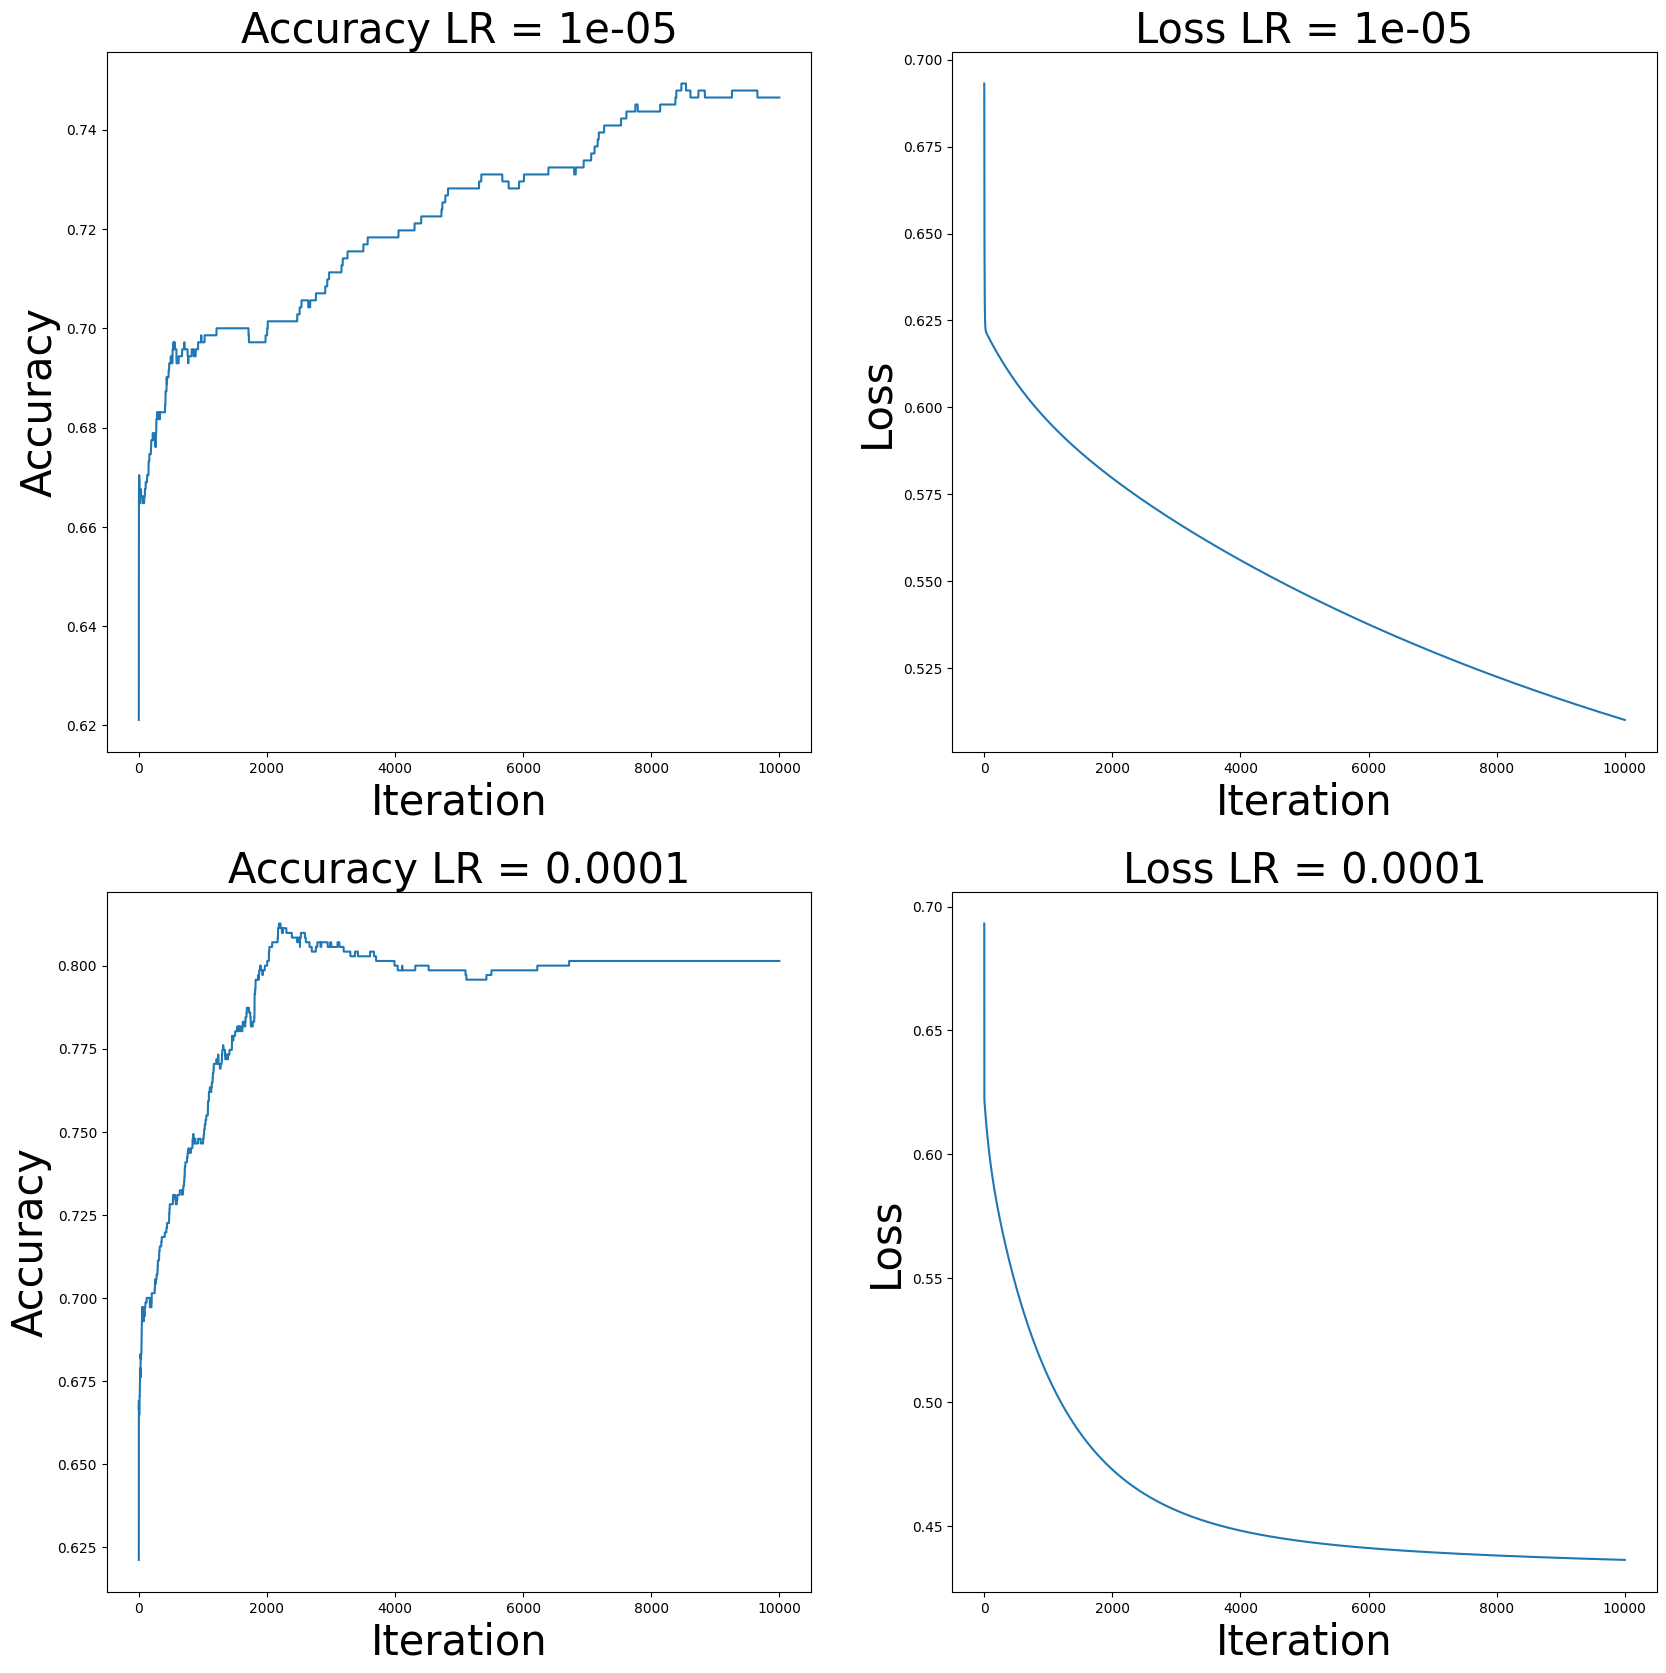
\includegraphics[width=\linewidth]{images/learning_rates_1.png}
    \label{fig:image1}
  \end{subfigure}
  \begin{subfigure}{0.3\linewidth}
    \centering
    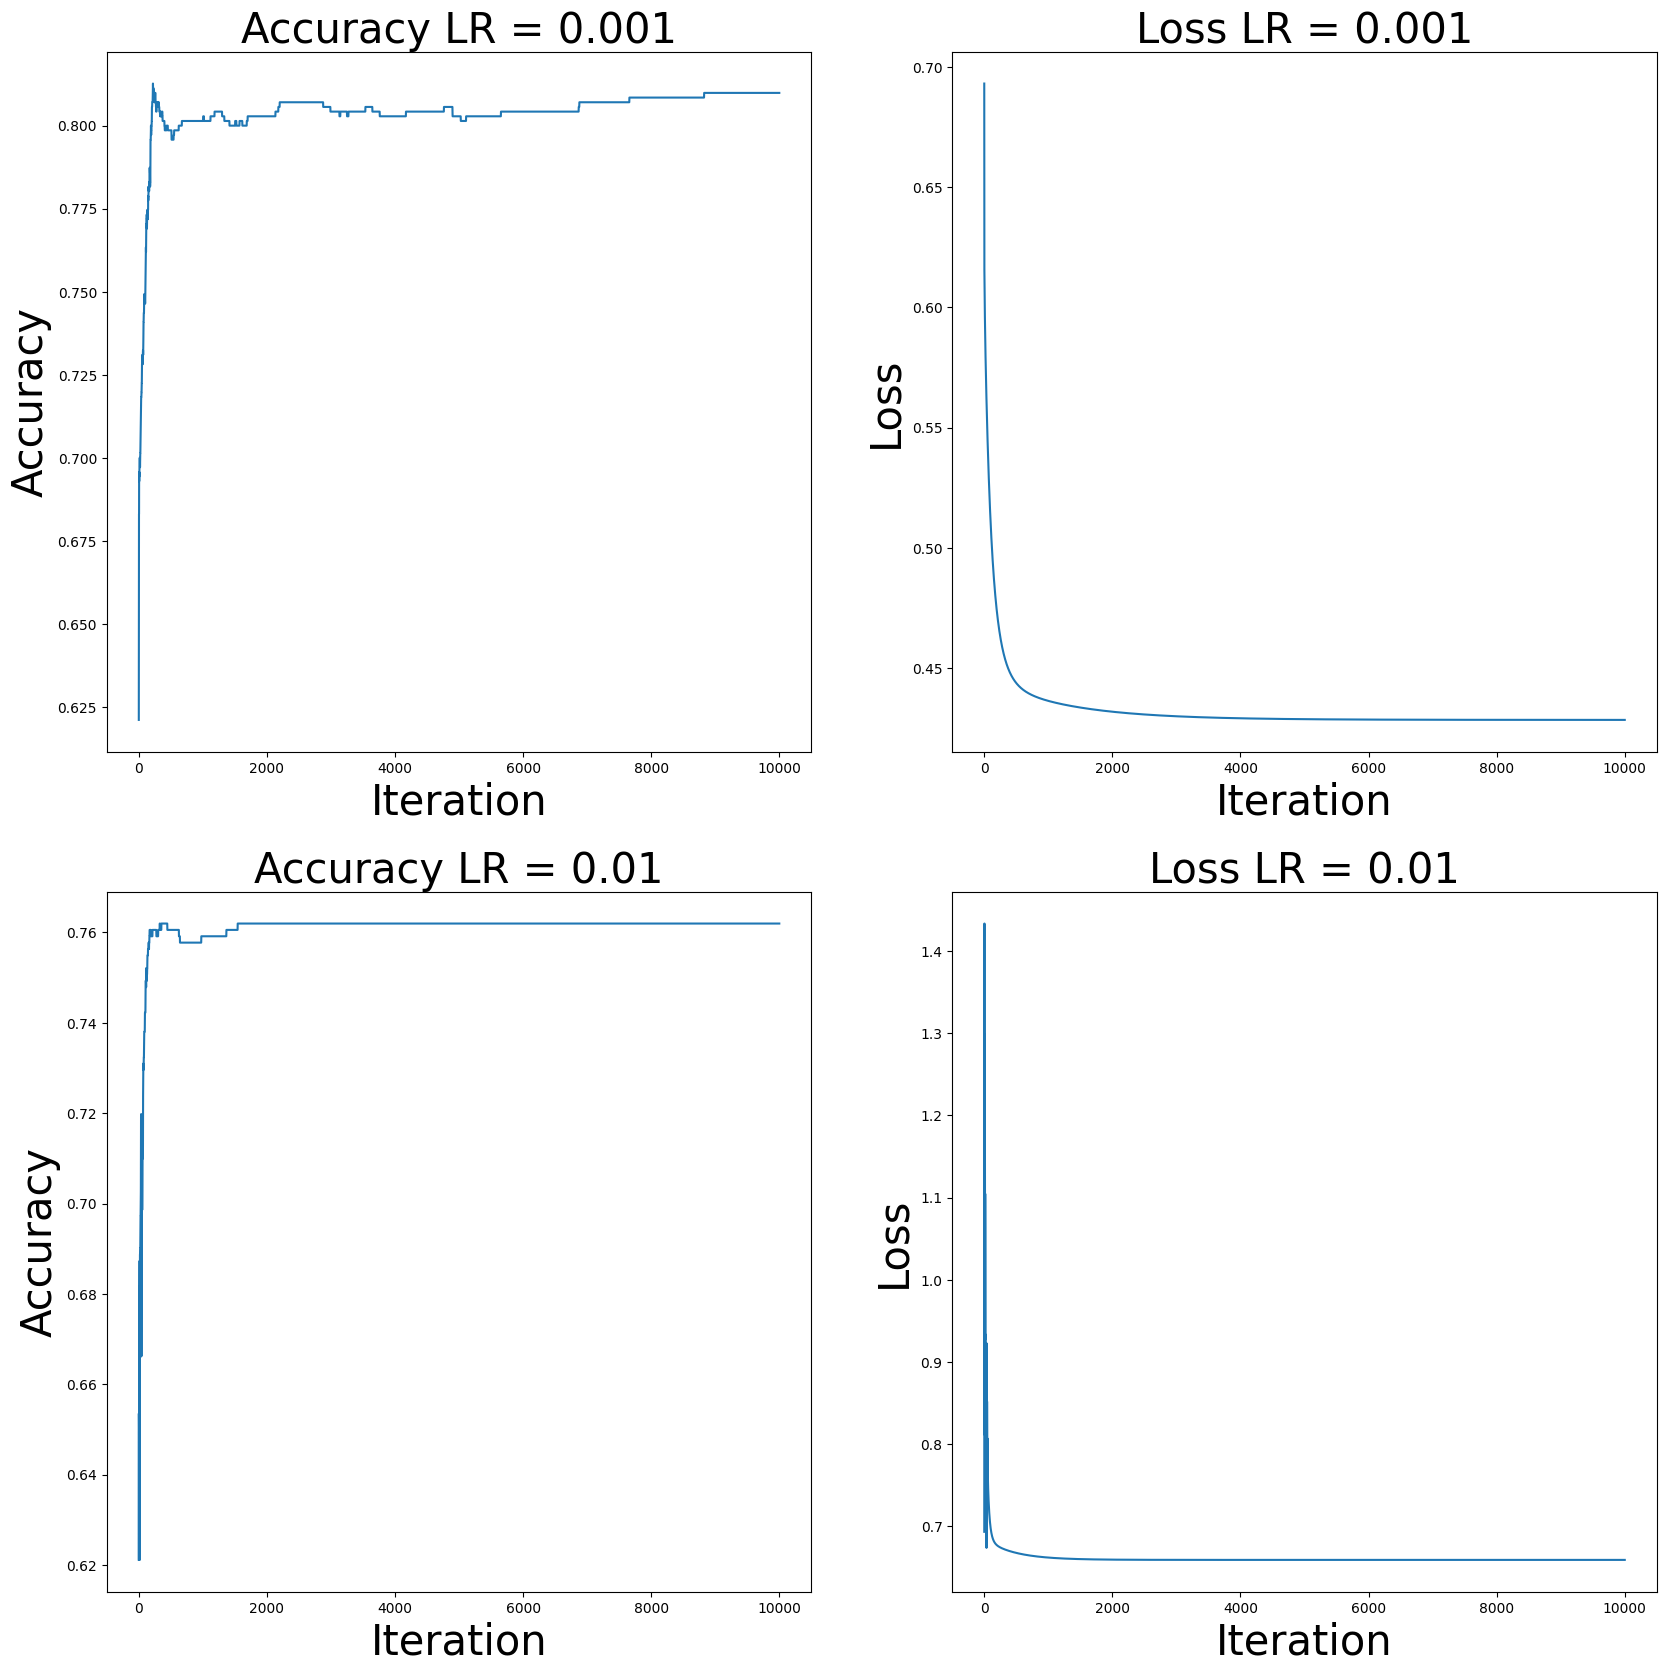
\includegraphics[width=\linewidth]{images/learning_rates_2.png}
    \label{fig:image2}
  \end{subfigure}
  \begin{subfigure}{0.3\linewidth}
    \centering
    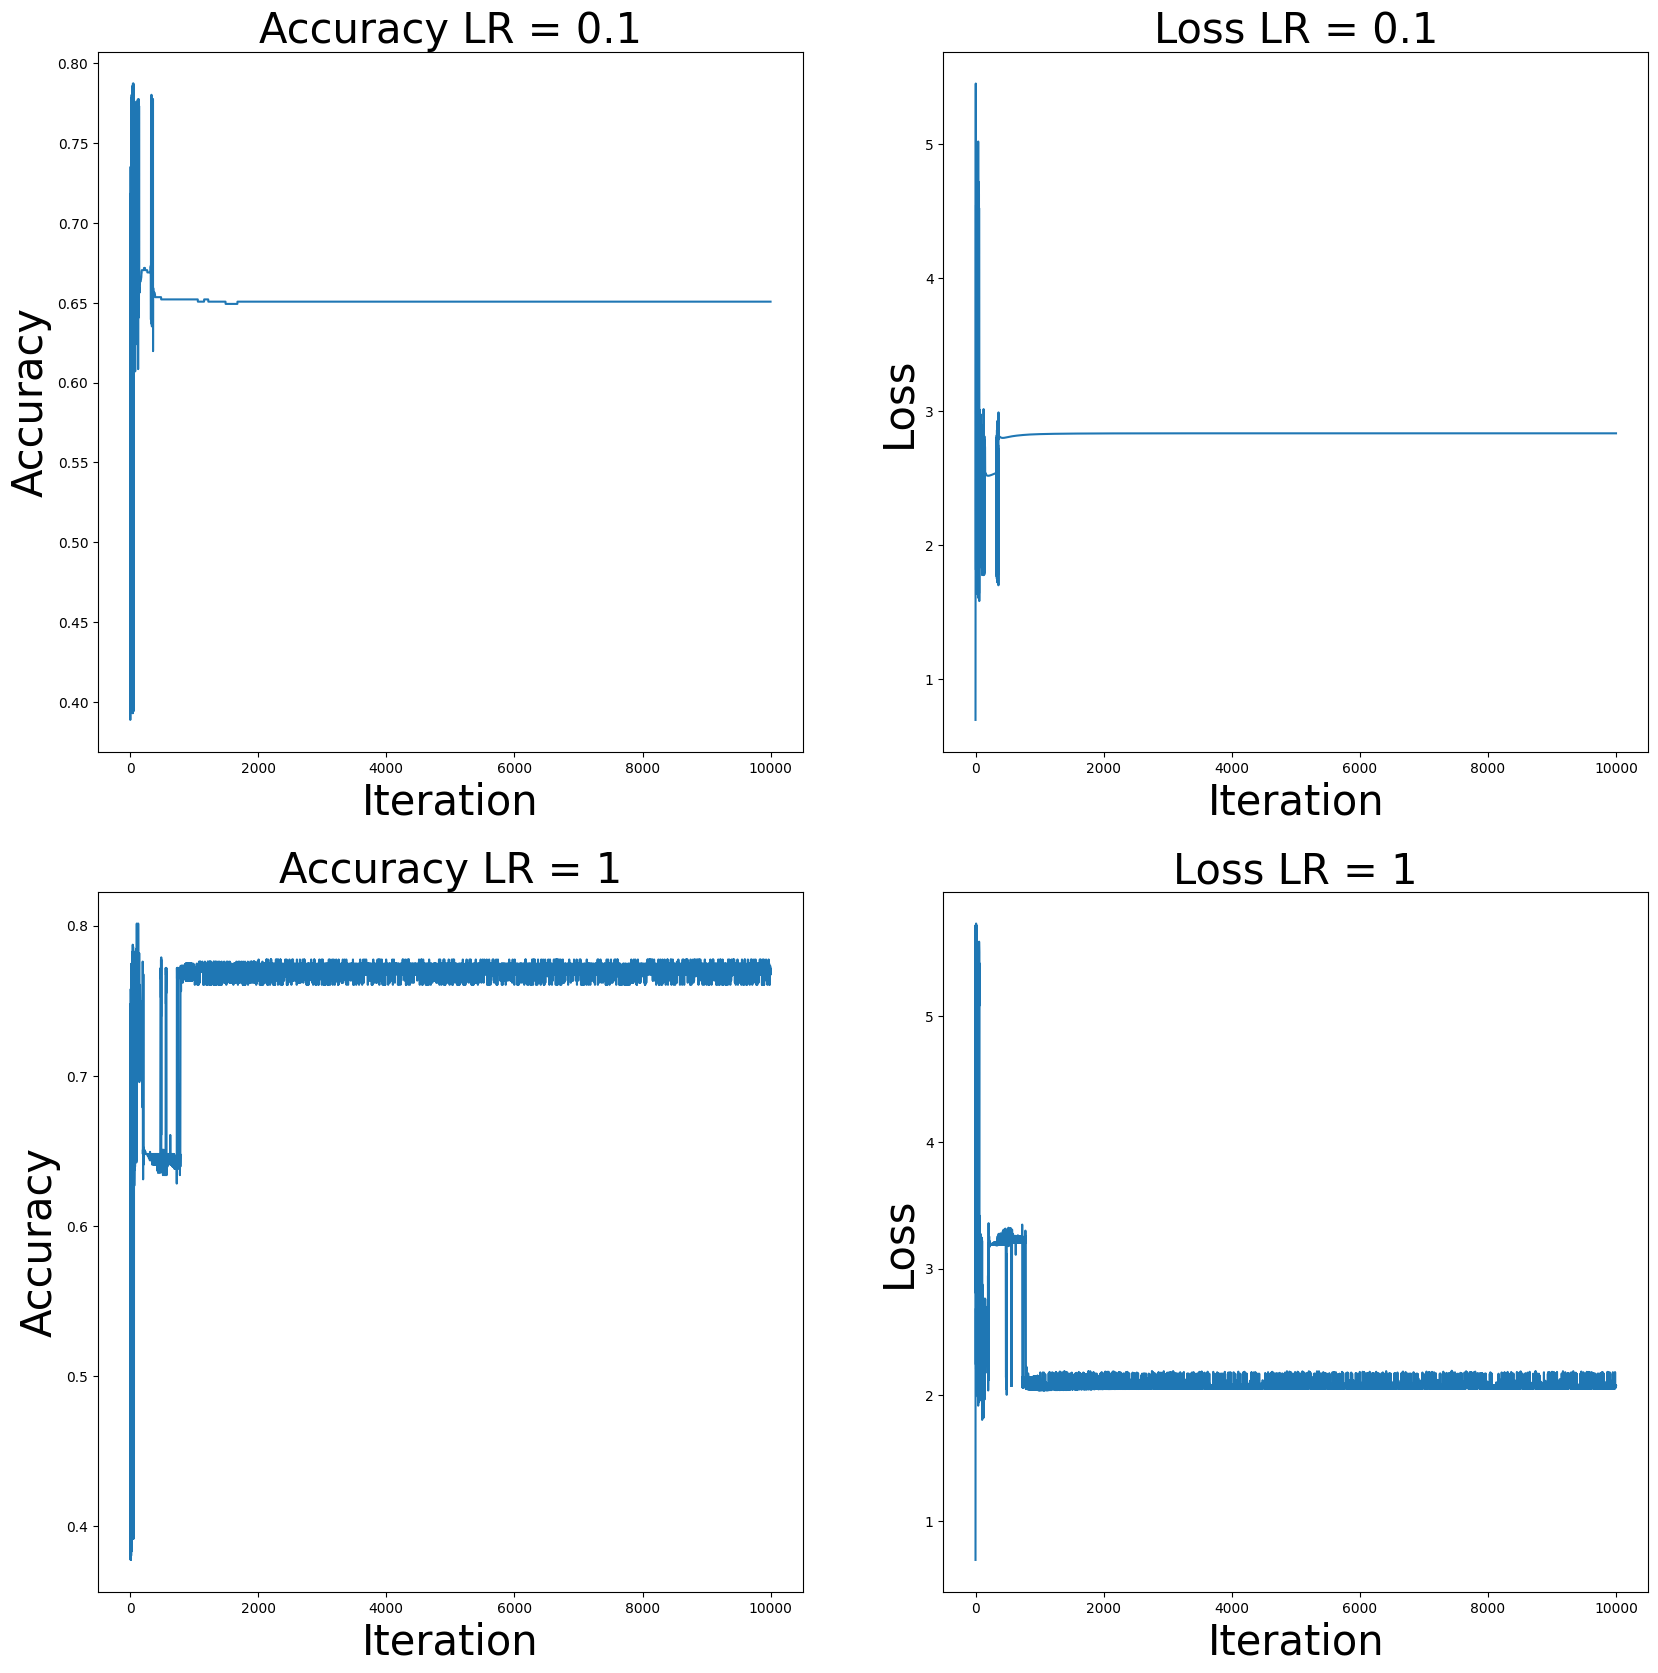
\includegraphics[width=\linewidth]{images/learning_rates_3.png}
    \label{fig:image3}
  \end{subfigure}
  \caption{Accuracy and Loss for different learning rates}
  \label{fig:three_images}
\end{figure}
\subsection{How many iterations are required to converge?}
To identify the number of iterations required for convergence,
it is enough to look at the accuracy and loss graphs at each iteration (figure \ref{fig:train_acc_loss}).
It converges when accuracy or loss does not decrease, or decrease by a negligible amount, as the number of iterations increases.
In this case, it converges after approximately 70 000 iterations.



\begin{figure}[h]
  \centering
  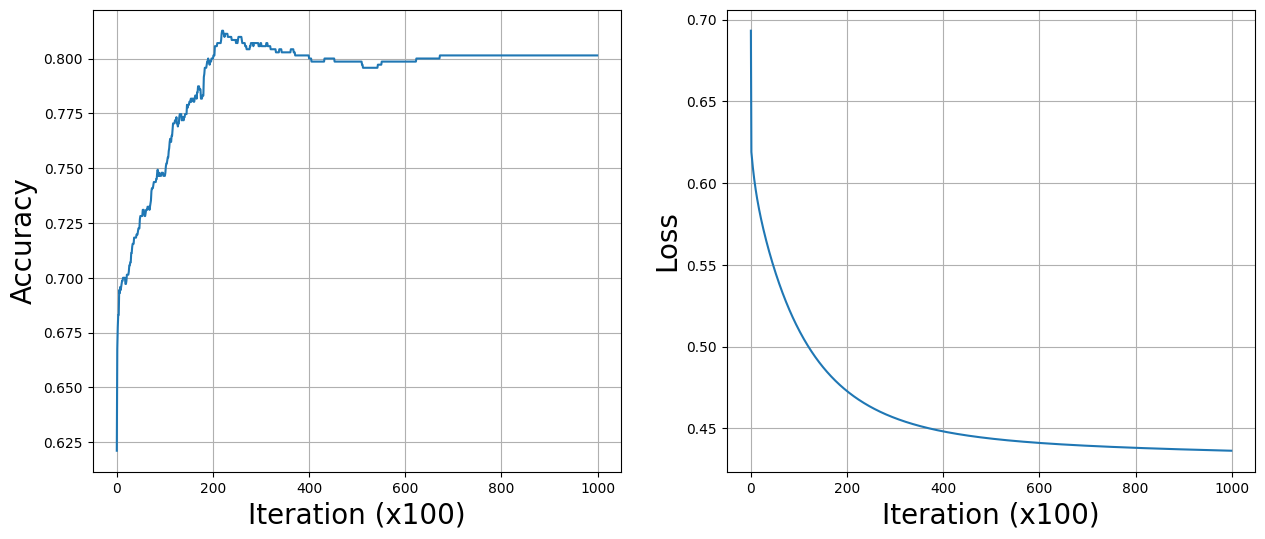
\includegraphics[width=0.6\textwidth]{images/Train_graphs.png}
  \caption{Accuracy and average crossentropy at each iteration}
  \label{fig:train_acc_loss}

\end{figure}

\clearpage

\section{Analyze the model}
\subsection{What would be my probability to survive? }
I am a 24-year-old male.
I would have purchased a first-class ticket for no more than 91 € and traveled with my girlfriend.
Below  the sample I provided, which has a 42.75\% chance of survival.

\bgroup
\rowcolors{2}{green!8}{green!18}
\begin{table}[h]
  \center
  \begin{tabular}{cccccc}
    Class & Sex & Age & N spouses & N parents & Fare \\
    \hline
    1     & 0   & 24  & 1         & 0         & 91   \\
  \end{tabular}
  \label{table:my_data}
  \caption{My information as a titanic passenger}
\end{table}
\egroup
\subsection{What is the training accuracy of the trained model?}
The training accuracy is  80.14\%.
The model used to get this result was trained with 1000000 iterations and a learning rate of 0.001
\subsection{Looking at the learned weights, how the individual features influence the probability of surviving?}
To analyze the impact of features on the probability of survival, we can examine their weights.
A higher coefficient value indicates a greater impact of the feature on the probability.
Moreover, if the weight is positive, increasing the feature value will cause the probability to increase as well.
Conversely, if the weight is negative, increasing the value of the feature will lead to a decrease in probability.
The figure \ref*{fig:parameters} shows that the ticket class and sex have the most significant impact on the probability,
while the age of the passenger and fare have a negligible effect.

\begin{figure}[h]
  \centering
  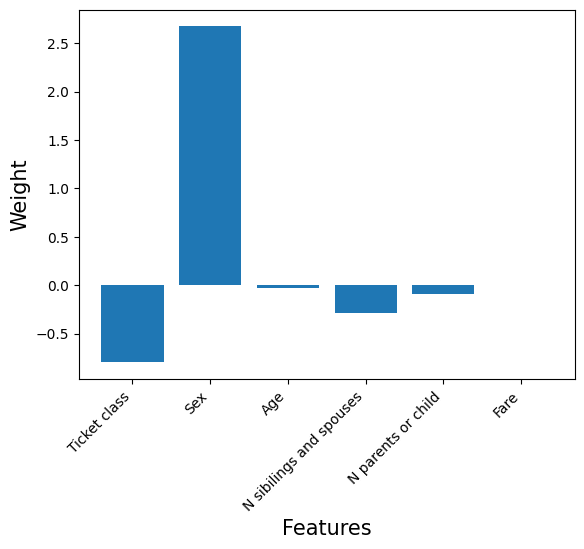
\includegraphics[width=0.3\textwidth]{images/Parameters.png}
  \caption{weight of the parameters}
  \label{fig:parameters}

\end{figure}

\subsection{What kind of passengers was most likely to survive? And what kind to to die?}
Based on the bar chart presented above, it is evident that women who were traveling in first class
and did not have any siblings or spouses accompanying them were more likely to survive.
Conversely, men who were in lower classes and had siblings or spouses with them were more likely to perish.

\clearpage

\subsection{Draw a scatter plot showing the distribution of the two classes in the plane defined by the two most influential features. Comment the plot.}
The graph displays the distribution of survivors (in yellow) and fatalities (in purple) by gender and ticket class.
It is evident that many women survived across all classes,
except for a considerable number of deaths in the third class.
Conversely, most men perished in all classes, except for a small number who survived in the first class.

\begin{figure}[h]
  \centering
  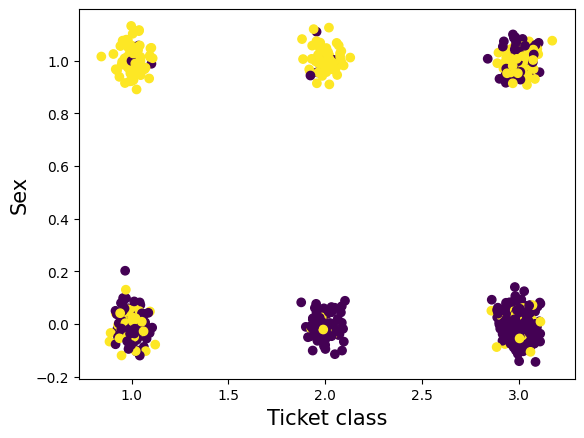
\includegraphics[width=0.3\textwidth]{images/Scatter_Sex_Class.png}
  \caption[Passengers grouped by the most significant features; The yellow points are the survived peoples and in purple the died ones]
  {\tabular[t]{@{}l@{}}Passengers grouped by the most significant features\\ The yellow points are the survived peoples and in purple the died ones\endtabular}
  \label{fig:scatter}

\end{figure}
\clearpage

\section{Evaluate the model}
\subsection{What is the test accuracy of the model?}
The test accuracy: 79.09\%
\subsection{Is the model overfitting or underfitting the training set?}
The model is well-suited for the data since both the test and train accuracy hover around 80\%,
indicating neither overfitting nor underfitting.
This high level of accuracy suggests that the model is effectively describing the data.


\subsection{How can you increase the performance of the model?}
The model's performance can be improved by increasing the number of training samples or applying regularization techniques.
With more training samples, the model can learn more about the data and make better predictions.
Regularization techniques, such as L1 or L2 regularization,
can prevent overfitting by reducing the impact of less significant parameters in the model.
Furthermore, to improve the computational performance of the model,
stochastic gradient descent (SGD) or mini-batch gradient descent (MBGD) can be used.
SGD updates the model parameters using only one sample at a time, while MBGD updates the parameters using a small batch of samples at a time.
MBGD is preferred over SGD because it is more regular and provides better convergence to the minimum of the loss function.
Additionally, MBGD can be easily parallelized, allowing for faster computations on parallel processing units such as GPUs.
Overall, these techniques can help improve both the accuracy and efficiency of the model.

\section{Declaration}
I affirm that
this report is the result of my own work and that I did not share any part of it with
anyone else except the teacher
\end{document}